\documentclass{llncs}
\usepackage[T1]{fontenc}
\usepackage{amsmath,amssymb}
\usepackage{graphicx}
\usepackage{booktabs}
\usepackage{url}
\usepackage{tikz}
\usepackage{listings}
\usepackage{multirow}
\lstset{basicstyle=\ttfamily\small,breaklines=true,frame=single,columns=fullflexible,captionpos=b}

\begin{document}
\title{Traceable Executable Reasoning over Query-Time Knowledge Graphs for Table--Text Question Answering}
\author{Author Names to Be Added}
\institute{Affiliations and corresponding author email to be added}
\maketitle

\begin{abstract}
Answering questions over tables and text requires preserving structural context,
connecting evidence across sources, and applying the correct operations to
retrieved values. A plausible reasoning path does not establish that its
computation is correct or supported by the available evidence. We present
Online-KG, a retrieval-augmented question answering framework that constructs
a knowledge graph at query time and evaluates candidate reasoning paths through
program execution. A deterministic entity anchor resolves a table-derived
bridge entity from question constraints and uses it to supplement first-stage
passage retrieval. The framework maintains an executable entity--relation graph
and a parallel typed structural trace for tables and passages. Candidate paths
are translated into Python programs or typed numerical programs and executed
through a restricted graph interface that records evidence access. An
evidence-aware selector combines execution outcomes, source support, and
agreement among candidate answers. Each prediction exports retrieval decisions,
the selected program, evidence, and path-level diagnostics for audit. We design
a controlled evaluation on HybridQA, FinQA, and HiTab to examine retrieval,
table structure, executable reasoning, and candidate selection alongside their
computational cost. Execution success, evidence access, and the exported
score-derived confidence remain diagnostic signals rather than guarantees of
answer correctness.
% Add a quantitative findings sentence after completing controlled experiments.
\keywords{Knowledge graphs \and Retrieval-augmented generation \and Executable reasoning \and Table question answering}
\end{abstract}

\section{Introduction}
Question answering over structured and unstructured information requires a
system to connect facts expressed in different forms. A table locates a value
through its row, column, and potentially several levels of headers, whereas a
passage expresses relationships through natural language. These sources can
play complementary roles: a table may report an earlier financial value while
a nearby sentence describes a subsequent change. HybridQA studies questions
requiring evidence from tables and linked passages~\cite{hybridqa}; FinQA
focuses on numerical reasoning over financial reports~\cite{finqa}; and HiTab
examines reasoning over hierarchical tables~\cite{hitab}. Together, these tasks
motivate systems that connect evidence while retaining the structure needed to
interpret it.

Consider a question asking for the percentage increase from a dividend listed
in a table to a newly declared dividend mentioned in text. Answering it requires
identifying the appropriate year and dividend column, linking the two values
to the same company, and computing the change relative to the earlier value.
Selecting a neighboring price column or reversing the denominator produces a
wrong answer even when the arithmetic executes successfully. Conversely,
finding the right operands is insufficient if the generated response applies
the wrong operation. This example separates three requirements: preserving
source context, composing evidence, and checking the resulting computation.

A retrieval-augmented system that passes evidence to a language model must
still determine how the evidence supports the answer. If table cells are
serialized without their full header context, their intended meaning can
become ambiguous. A graph provides an explicit representation of relationships,
but graph connectivity alone does not specify how to calculate a percentage
change, aggregate values, or compare alternatives. Similarly, agreement among
several generated answers can reflect repeated use of the same mistaken
operand. These considerations motivate candidate evaluation that examines both
execution behavior and the evidence consulted during execution.

We present Online-KG, a framework organized around the sequence
\emph{construct, plan, execute, and select}. For each question, the system
constructs a graph from the supplied table and retrieved passages.
Deterministic structural triples retain row identities and column context,
including hierarchical header paths where available. Before passage enrichment,
a deterministic anchor can resolve a bridge entity from a table constraint, such
as a rank, and retrieve its associated passage. Semantic triples add
relationships extracted from the accompanying content, and edge provenance
records their sources. A parallel typed trace retains table, row, column, cell,
and passage topology for audit without changing the executable graph API.
Here, ``online'' refers to construction at query time; it does not imply
continual training or access to live web information.

The system then generates multiple candidate reasoning paths and translates
them into executable Python programs. Programs access the graph through a
restricted interface, allowing the executor to record the graph edges they
consult. Candidate selection uses execution outcomes, evidence support, source
diversity, and answer agreement. The central design choice is to evaluate
candidate computations after execution, with access to their outputs and
recorded evidence, instead of choosing solely from textual plans. A typed
numerical intermediate representation provides a complementary execution
variant with explicit lookup and arithmetic operations. Neither successful
execution nor a record of evidence access is treated as proof that a candidate
correctly answers the question.

Our study asks whether this combination improves answer quality under matched
context and model settings, which components account for any observed changes,
and what computational cost they introduce. We plan controlled comparisons on
HybridQA, FinQA, and HiTab, covering heterogeneous evidence, numerical
computation, and hierarchical table structure. Initial experiments use
benchmark-supplied tables and associated context; their scope is reasoning
within that context rather than open-domain retrieval. Comparisons include
direct answering, graph paths without code execution, agreement-only selection,
and alternative executable representations.

The paper develops four methodological contributions:
\begin{itemize}
    \item A two-stage retrieval procedure that uses inspectable question
    constraints to identify table-derived bridge entities, followed by
    entity-centered passage supplementation.
    \item A query-time graph construction procedure combining structural table
    triples and semantic evidence, with a parallel typed topology trace and
    edge provenance available for audit.
    \item An executable reasoning pipeline that converts candidate graph paths
    into programs and records their outputs and consulted graph evidence.
    \item An evidence-aware candidate selection mechanism and prediction trace
    that expose source support, executed paths, and answer diagnostics for
    controlled comparison with selection based on agreement alone.
\end{itemize}
% Finalize empirical contribution claims only after evaluating matched runs.

\section{Related Work}
\label{sec:related}
\paragraph{Table--text and table retrieval.}
HybridQA established a setting in which a question requires a Wikipedia table
and passages linked from table entities~\cite{hybridqa}. FinQA couples financial
tables, report text, and executable gold programs~\cite{finqa}; HiTab tests
hierarchical tables with nested row and column headers~\cite{hitab}. These
benchmarks expose a limitation of flattening a table into a text prompt: a cell
can lose its row, column, and header context. TableRAG for large-scale table
understanding retrieves schemas and cells after query expansion, reducing the
prompt footprint for very large tables~\cite{chen2024tablerag}. A different
TableRAG formulation uses text retrieval, SQL generation and execution, and
intermediate-answer composition for heterogeneous documents~\cite{yu2025tablerag}.
Our method shares their premise that table structure should influence retrieval
and reasoning. It differs in scope: it constructs a compact per-query graph
from supplied benchmark context, preserves structural provenance in a parallel
trace, and evaluates several executable graph-path candidates rather than using
SQL as the sole table interface. This is a design comparison, not a claim of
superiority; the experiments in Section~\ref{sec:experiments} control the
available context and model configuration.

\paragraph{Graph-enhanced RAG.}
Graph-based retrieval can expose multi-hop relations that text similarity alone
may miss. HydraRAG combines pre-existing KG, Wikipedia, and web sources through
agentic exploration and tri-factor verification based on source trustworthiness,
cross-source corroboration, and entity-path alignment~\cite{tan2025hydrarag}.
Its evidence graph is assembled from external Freebase/Wikidata services and
documents during exploration. Online-KG instead creates its executable graph
from the table and passage context for the current question. It consequently
does not require a global KG service, but it also does not provide HydraRAG's
coverage over external sources or its source-trustworthiness model. The two
systems share the use of provenance and multi-source evidence, while their graph
construction time, source assumptions, and verification mechanisms differ.

\paragraph{Executable reasoning and candidate selection.}
Program-aided language models delegate deterministic computation to an
interpreter after an LM generates code~\cite{gao2023pal}; program-of-thought
prompting similarly separates numerical computation from natural-language
reasoning~\cite{chen2022pot}. For table QA, executable representations such as
SQL~\cite{yu2025tablerag} or the programs annotated in FinQA~\cite{finqa} make
operations inspectable. These approaches motivate executing rather than merely
describing an arithmetic plan. Online-KG adds two restrictions that matter for
the present setting: generated code can only access a limited graph API, and
the executor records the KG edges returned by those calls. The system then ranks
multiple executed candidates using source support and output agreement. Execution
removes arithmetic errors conditional on selected operands, but it cannot show
that those operands or the operation answer the question; the contrasting paths
in Figure~\ref{fig:kg-paths} make this limitation explicit.

\section{Problem Formulation}
Given a question $q$, a table $T$, and associated passages $D$, the system
produces an answer $a$ and an execution trace. In the initial benchmark setting,
$T$ and the associated passage pool are provided by the dataset. Passage ranking
therefore operates within supplied context; this is not an evaluation of
open-domain retrieval. The graph $G_q$ is constructed separately for each query.

\begin{figure}[t]
\centering
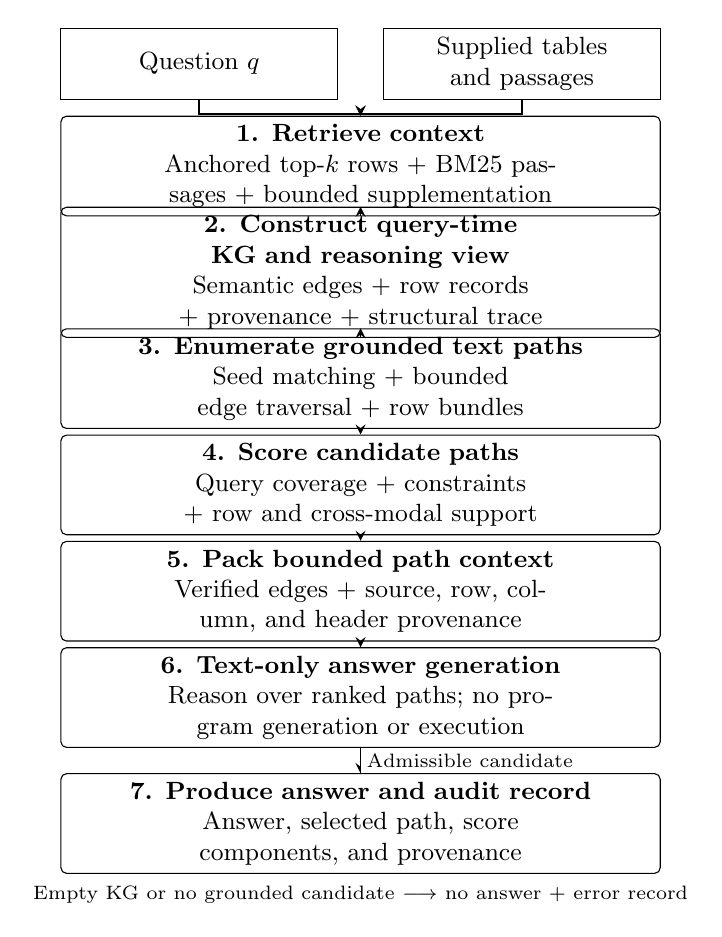
\begin{tikzpicture}[
  >=stealth,
  stage/.style={draw,rounded corners=2pt,align=center,text width=7.4cm,
    minimum height=9mm,inner sep=3pt,font=\small},
  source/.style={draw,align=center,text width=3.3cm,
    minimum height=9mm,inner sep=3pt,font=\small},
  flow/.style={->,line width=0.6pt},
  note/.style={font=\scriptsize,align=center,fill=white,inner sep=2pt}
]
\node[source] (question) at (-2.05,0)
  {Question $q$};
\node[source] (sources) at (2.05,0)
  {Supplied tables and passages};

\node[stage] (retrieve) at (0,-1.3)
  {\textbf{1. Retrieve context}\\
   Anchored top-$k$ rows + BM25 passages + bounded supplementation};
\node[stage] (build) at (0,-2.65)
  {\textbf{2. Construct query-time KG and reasoning view}\\
   Semantic edges + row records + provenance + structural trace};
\node[stage] (plan) at (0,-4)
  {\textbf{3. Enumerate grounded text paths}\\
   Seed matching + bounded edge traversal + row bundles};
\node[stage] (synth) at (0,-5.35)
  {\textbf{4. Score candidate paths}\\
   Query coverage + constraints + row and cross-modal support};
\node[stage] (execute) at (0,-6.7)
  {\textbf{5. Pack bounded path context}\\
   Verified edges + source, row, column, and header provenance};
\node[stage] (select) at (0,-8.05)
  {\textbf{6. Text-only answer generation}\\
   Reason over ranked paths; no program generation or execution};
\node[stage] (answer) at (0,-9.65)
  {\textbf{7. Produce answer and audit record}\\
   Answer, selected path, score components, and provenance};

\draw[flow] (question.south) -- ++(0,-0.18) -| (retrieve.north);
\draw[flow] (sources.south) -- ++(0,-0.18) -| (retrieve.north);
\draw[flow] (retrieve) -- (build);
\draw[flow] (build) -- (plan);
\draw[flow] (plan) -- (synth);
\draw[flow] (synth) -- (execute);
\draw[flow] (execute) -- (select);
\draw[flow] (select) -- node[note,right] {Admissible candidate} (answer);

\node[note] at (0,-10.55)
  {Empty KG or no grounded candidate $\longrightarrow$ no answer + error record};
\end{tikzpicture}

\caption{Overview of Online-KG. Retrieval and graph construction run once per
question. Candidate plans are converted to Python programs or, in the numerical
variant, typed IR programs. Execution returns outputs and accessed-edge evidence
for candidate selection. The dashed loop generates fresh plans over the same
graph when no candidate is admissible, subject to a replanning budget. Python
mode additionally permits a symbolic-search fallback before replanning
(omitted from the diagram).}
\label{fig:pipeline}
\end{figure}

\section{Method}
\label{sec:method}

\subsection{Overview}
Given a question $q$, supplied tables $\mathcal{T}$, and an associated passage
pool $\mathcal{D}$, the method constructs a bounded knowledge graph specifically
for $q$. The graph is an intermediate reasoning structure rather than a
persistent database. The pipeline is
\[
q \rightarrow \text{row and passage retrieval}
\rightarrow \text{local KG construction}
\rightarrow \text{grounded text paths}
\rightarrow \text{path ranking}
\rightarrow \text{answer}.
\]
No program generation or execution is required by the primary method. Python
and typed numerical programs remain separate experimental variants.

\subsection{Query-Driven Context Retrieval}
A deterministic anchor first inspects the question and table schema. Its current
rules recognize ordinal constraints, exact numerical table constraints, and a
small set of entity-bearing columns. An ordinal such as \emph{second} can
therefore identify a bridge entity from a rank--entity row even when that entity
does not occur in the question.

Table retrieval forms a union of anchor-matched rows and BM25-ranked rows, with a
global row budget $k$. Original row indices are retained after filtering. This
is important because the same label can occur in several rows and because
provenance must refer to the source table rather than the filtered position.
Passage retrieval first applies BM25 to $q$, then adds at most $b$ passages using
bridge-entity queries and deterministic schema expansions. Duplicate passages
are removed by source identifier. The current defaults are $k=5$ and $b=3$ in
the benchmark runner; experiments record any override.

The benchmark setting supplies an oracle table and its associated passage pool.
Retrieval is therefore query-local within supplied context, not open-domain
table or web search.

\subsection{Schema-Preserving Online KG Construction}
For each question, the system creates a directed multigraph
$G_q=(V_q,E_q)$. A semantic edge is
\[
e=(h,r,t,\pi),
\]
where $h$ and $t$ are entity or literal labels, $r$ is a normalized relation,
and $\pi$ stores source type, source identifier, and optional row, column, and
header-path metadata. A multigraph retains separate provenance records when
several sources express the same fact.

\paragraph{Deterministic table edges.}
Dataset adapters convert a selected row into a dictionary with a row label and
qualified column names. The first nonempty field supplies the row subject
$u_i$; every other nonempty cell produces
\[
(u_i,\operatorname{norm}(H_j),v_{ij},\pi_{ij}).
\]
Hierarchical headers are qualified before graph construction. For example,
\texttt{2002 / Dividend} becomes \texttt{2002\_dividend}, preventing a
dividend from being confused with \texttt{2002\_high}.

Direct subject--value edges are convenient for entity lookup but do not by
themselves preserve which values co-occur in one row. The path-text reasoning
view therefore adds a record node $\rho_i$:
\[
u_i \xrightarrow{\mathrm{has\_record}} \rho_i, \qquad
\rho_i \xrightarrow{\operatorname{norm}(H_j)} v_{ij}.
\]
For two records of the same company, this representation prevents a year from
one row being paired with a revenue from another. Record identifiers are local
implementation nodes and do not alter the legacy executable entity interface.

In parallel, an audit trace stores
Table $\rightarrow$ Row $\rightarrow$ Cell $\rightarrow$ Column topology.
Thus the implementation exposes an entity-centric semantic graph, a
record-aware path view, and a complete structural trace without conflating their
roles.

\paragraph{Text edges and entity resolution.}
An LLM extracts semantic triples from each retrieved passage. A small set of
deterministic extractors preserves recurrent numerical and name facts when the
model response is malformed. Failed optional table enrichment falls back to
deterministic cells; a failed passage is logged and skipped. Entity resolution
then applies lexical normalization, configured aliases, structural name rules,
and conservative string similarity. Resolution events and rejected self-loops
are included in the trace.

The graph metadata distinguishes entity-oriented nodes, literal attributes, and
record structure operationally. It is not presented as a learned ontology or
a general semantic type system.

\subsection{Grounded Text-Path Generation}
The reasoning edge set $E_q^*$ is the union of semantic edges and row-record
edges. Candidate generation never invents an edge: every emitted path step
contains an edge identifier from $E_q^*$ together with direction and provenance.
Traversal may follow an edge forward or backward, but its stored factual
direction remains unchanged.

Seeds are graph nodes that match a question phrase, a bridge entity, or an
explicit table constraint. When no node is matched, endpoints of relations
sharing terms with the question provide fallback seeds. From each seed, bounded
search enumerates simple connected paths of at most three edges. Branching and
the total enumerated candidates are capped. The implementation additionally
creates a row bundle containing
$u_i\rightarrow\rho_i$ and the most question-relevant outgoing cell edges.
A row bundle is a connected evidence subgraph rather than a forced linear chain;
this allows a year constraint and requested value to remain attached to the same
record.

Each candidate is verbalized directly from its verified edges, for example
\[
\texttt{A --has\_record--> row:7 --year--> 2022}
\]
together with a sibling edge
\[
\texttt{row:7 --revenue--> 10M}.
\]
This differs from asking a language model to propose plausible relation names
from a list of nodes and relations.

\subsection{Text-Path Scoring}
All candidates pass a hard groundedness gate because generation only accepts
registered edge identifiers. The implemented heuristic score is
\[
\begin{split}
S(p)={}&G+Q_e+Q_r+Q_c+C+M+R+B+A\\
      &-0.35\max(|E_p|-1,0),
\end{split}
\]
where $G=1$ is grounded-edge validity; $Q_e$ and $Q_r$ are question overlap
with path nodes and relations, each capped at 2; and $Q_c$ is question-term
coverage, also capped at 2. The constraint term $C=2$ when the path includes
an anchored table value or allowed output candidate.

The cross-modal completeness term $M=1.5$ when a path uses both table and text
evidence. This is not called agreement: different sources may supply different
hops. Same-fact corroboration $A=1$ is awarded only when normalized
$(h,r,t)$ is supported by both table and text. Row consistency $R=1$ requires
at least two record-aware edges from one source row, and entity binding $B=1$
additionally requires the \texttt{has\_record} edge. These weights are fixed
heuristics rather than learned probabilities.

The top $N$ distinct paths are serialized with their score components, nodes,
edges, source identifiers, row indices, columns, and header paths. Supporting
edges are packed within a character budget, with selected path edges receiving
priority. Context packing does not change the path scores.

\subsection{Answer Production and Audit Record}
The answer model receives only the ranked paths, supporting KG edges, table
constraints, and the question. It reasons over this evidence as text and returns
a short answer span; it is explicitly instructed not to generate or execute a
program. The output is canonicalized to a resolved KG alias and, when a table
constraint defines an allowed candidate set, to the corresponding exact table
value.

Each prediction records the retrieved row count, passage retrieval decisions,
entity anchor, KG summary, ranked paths, score decomposition, and selected path
identifier. Empty graphs or an empty candidate set produce an explicit failure
record rather than an unsupported answer.

The trace establishes that path edges exist in the constructed graph. It does
not prove that LLM-extracted text triples are factually correct, that the
retriever found all required evidence, or that the top-ranked grounded path is
semantically sufficient for the question.


\section{Experimental Protocol}
\label{sec:experiments}
\subsection{Datasets and Metrics}
We use the fixed development splits of HybridQA, FinQA, and HiTab, with versions,
file hashes, and exact example identifiers recorded in the released run manifest.
HybridQA evaluates table--text answer extraction with exact match (EM) and token
F1. FinQA reports its strict five-decimal execution metric as the primary score;
we report a ratio/percentage-equivalent metric only as a separately labelled
diagnostic. HiTab reports strict denotation accuracy on its original scale and,
separately, a ratio/percentage-normalized diagnostic. Python-path correctness is
not presented as official FinQA program accuracy. FinQA experiments using its
normalized official table and its raw hierarchical table are separate protocols.

\subsection{Baselines and Ablations}
The benchmark suite compares direct LLM answering, flattened-table BM25,
Online-KG path text without code, path-consistency selection, typed numerical
IR, and the full Python Online-KG pipeline. All methods use the same supplied
context, model, decoding configuration, and answer budget within each run.
Our ablations remove the second retrieval stage, bridge-entity queries,
structural table triples, semantic enrichment, header hierarchy, or
evidence-aware selection. Each configuration is run only after its implementation
is verified. We report anchor coverage and bridge-entity passage recall on the
subset where an anchor applies; retrieving a bridge entity does not ensure a
correct final answer.

\subsection{Controls and Cost}
Fix example identifiers, model version, decoding settings, context limits, and
retrieval settings across comparable methods. Record candidate count, replanning
budget, fallback policy, API attempts, logical model calls, and wall time.
Use measured provider token usage if available; missing usage is not zero.
Report paired uncertainty estimates and failure rates on a fixed evaluation set.
Archive retrieval traces, typed structural traces, selected-path metrics, and
the repository revision. Treat the exported confidence as an uncalibrated
diagnostic; do not evaluate it as calibrated confidence without a dedicated
calibration study.

\section{Results and Error Analysis}
\label{sec:results}
This section is a camera-ready results scaffold. Cells marked \texttt{TBD} must
be replaced only from completed, fixed-configuration runs; no conclusions should
be drawn until Table~\ref{tab:main-results} is filled. Each reported row must
name the dataset split, model identifier, repository revision, prompt version,
and decoding configuration in the accompanying run manifest.

\begin{table}[t]
\caption{Main benchmark results. Fill one block per dataset from the fixed run
manifest. Report mean latency and logical LLM calls per example on the same
evaluation records used for accuracy. Higher is better for all accuracy metrics.}
\label{tab:main-results}
\centering
\scriptsize
\begin{tabular}{llrrrr}
\toprule
Dataset & Method & Primary metric & Secondary metric & Calls & Latency (s) \\
\midrule
HybridQA & Direct LLM & \texttt{TBD} EM & \texttt{TBD} F1 & \texttt{TBD} & \texttt{TBD} \\
         & Flat-table BM25 & \texttt{TBD} EM & \texttt{TBD} F1 & \texttt{TBD} & \texttt{TBD} \\
         & Online-KG path text & \texttt{TBD} EM & \texttt{TBD} F1 & \texttt{TBD} & \texttt{TBD} \\
         & Online-KG (Python) & \texttt{TBD} EM & \texttt{TBD} F1 & \texttt{TBD} & \texttt{TBD} \\
\midrule
FinQA    & Direct LLM & \texttt{TBD} official exec. & \texttt{TBD} ratio/\% & \texttt{TBD} & \texttt{TBD} \\
         & Numerical IR & \texttt{TBD} official exec. & \texttt{TBD} ratio/\% & \texttt{TBD} & \texttt{TBD} \\
         & Online-KG (Python) & \texttt{TBD} official exec. & \texttt{TBD} ratio/\% & \texttt{TBD} & \texttt{TBD} \\
\midrule
HiTab    & Numerical IR & \texttt{TBD} strict den. & \texttt{TBD} normalized & \texttt{TBD} & \texttt{TBD} \\
\bottomrule
\end{tabular}
\end{table}

\begin{table}[t]
\caption{Ablation and audit template. Evaluate all rows on the same anchorable
subset for bridge retrieval, and use the same completed examples for answer
metrics. ``Bridge recall'' is not applicable to a table-only dataset.}
\label{tab:ablations}
\centering
\scriptsize
\begin{tabular}{lrrrr}
\toprule
Configuration & Primary metric & Anchor coverage & Bridge recall & Cross-modal paths \\
\midrule
Full Online-KG & \texttt{TBD} & \texttt{TBD} & \texttt{TBD} & \texttt{TBD} \\
No second stage ($b=0$) & \texttt{TBD} & \texttt{TBD} & \texttt{TBD} & \texttt{TBD} \\
No bridge-entity query & \texttt{TBD} & \texttt{TBD} & \texttt{TBD} & \texttt{TBD} \\
No structural triples & \texttt{TBD} & \texttt{TBD} & \texttt{TBD} & \texttt{TBD} \\
Agreement-only selector & \texttt{TBD} & \texttt{TBD} & \texttt{TBD} & \texttt{TBD} \\
\bottomrule
\end{tabular}
\end{table}

\paragraph{Analysis protocol.}
After filling the tables, report paired bootstrap confidence intervals for the
difference between the full system and its strongest matched baseline. Partition
failures into retrieval/anchor, table parsing or header interpretation, entity
resolution, program syntax or schema, operand selection, operator composition,
arithmetic execution, unit/scale, and answer rendering. For numerical IR, also
report parse validity, schema validity, execution success, operator accuracy,
step accuracy, and grounding precision/recall where gold annotations permit.
Do not merge unavailable metrics into an error category.

\paragraph{Case-study template.}
Select one correct and one incorrect held-out example after evaluation. For each,
show the question, retrieved sources and anchor, relevant structural cells,
executable graph edges, candidate programs, executed values, selected-path
score, and final answer. State whether the trace explains an error or merely
records access. The constructed example in Figure~\ref{fig:kg-paths} illustrates
the presentation format and is not a substitute for held-out evidence.

\section{Limitations}
The current experiments assume dataset-supplied tables and, for FinQA, the
associated report context; they therefore do not measure open-domain table or
document retrieval. HiTab is evaluated as hierarchical table-only QA, so it
tests structural and numerical reasoning but cannot demonstrate table--text
provenance diversity. The deterministic table graph preserves row and column
header paths, but graph size grows with the number of cells, while optional LLM
enrichment can introduce redundant parallel edges or noisy relations.

The numerical IR currently covers a practical but incomplete operator set.
Questions involving ranking, ranges, dates, complex percentages, implicit unit
conversion, or domain-specific financial operators may require additional
operators or repair. A successfully executed program is not necessarily a
semantically correct one: it may select the wrong grounded cells, reverse an
ordered subtraction, or apply a valid operator to an incorrect set of values.
Consequently, execution success is reported separately from denotation,
operator, step, and grounding accuracy. Step-level evaluation also depends on
the availability and alignment of gold programs and is not directly comparable
across datasets with different annotation conventions.

Planning and graph enrichment still require multiple model calls, increasing
latency and exposing results to provider failures and model variance. Source
counts are only an approximation of independence because different passages or
edges may repeat the same underlying fact. Full graph traces improve
auditability but can become visually dense and should not be treated as proof
that every extracted edge is correct. Finally, restricted Python execution is
an engineering sandbox rather than a formally verified security boundary.

\section{Conclusion}
This draft defines a study of executable reasoning over query-time table--text
graphs. Final conclusions will depend on controlled benchmark and ablation results.

\bibliographystyle{splncs04}
\bibliography{refs}
\end{document}
